\documentclass{beamer}

\usepackage{pgfpages}
% Note rendering settings
% \setbeameroption{hide notes} % Default
% \setbeameroption{show notes}
% \setbeameroption{show only notes}
% \setbeameroption{show notes on second screen}

% Maths
\usepackage{mathabx}
\usepackage{mathtools}

% Support for sane handling of values with SI units
\usepackage{siunitx}

% Algorithms using algorithmicx package (with its algpseudocode command set)
\usepackage{algpseudocode}

% Code listings
\usepackage{listings}
\usepackage{lstautogobble}
\lstset{
		basicstyle=\small,
		breaklines=true,
		autogobble=true,
		postbreak=\mbox{$\drsh$},
}

% Date management
\usepackage{datetime2}
\DTMsavedate{presentation}{2022-12-07}

% BibLaTeX
\usepackage[
  style=alphabetic,
  backend=biber, % Default backend, just listed for completness
  sorting=ynt % Sort by year, name, title
]{biblatex}
\addbibresource{references.bib}
% Main resource for presentation
\nocite{fisherPunchscanIntroductionSystem2006}

% A more modern (and less beamer-y) theme
\usetheme{metropolis}

% \metroset{sectionpage=simple}
% Optional light gray fill behind block environments such as \theorem
\metroset{block=fill}

\title{Punchscan}
\subtitle{Paper-based voting with E2E auditing capabilities}
\author{Michael Senn}
\institute{Faculty of Science, University of Bern}
\date{\DTMusedate{presentation}}

\begin{document}

\maketitle

\section{Motivation}

\begin{frame}{Motivation}
	To provide a voting system, where:
	\begin{itemize}
		\item The vote is managed by a central election authority
			\begin{itemize}
				\item But auditors provide resilience against a malicious election authority
			\end{itemize}
		\item Voters get a paper-based receipt
			\begin{itemize}
				\item Which does not allow votes to be bought nor coerced
				\item Yet allows them to verify their votes are cast-as-intended
			\end{itemize}
		\item Voters intuitively understand how to vote
		\item Thus: Punchscan, 2006 \autocite{fisherPunchscanIntroductionSystem2006}
	\end{itemize}
\end{frame}

\section{Ballot layout}

\begin{frame}{Ballot layout}
	\begin{itemize}
		\item Ballot consists of two pages, stacked on top of each other
		\item Both pages have serial number identifying ballot
	\end{itemize}
	\begin{figure}
		\centering
		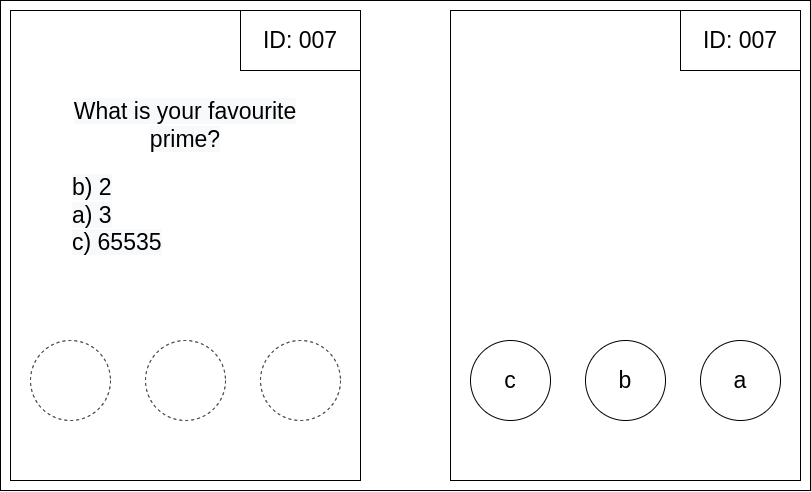
\includegraphics[width=0.65\textwidth]{../resources/high_level_ballot.drawio.png}
		\caption{Top (left) and bottom (right) halves of ballot}
	\end{figure}
\end{frame}

\begin{frame}{Ballot layout: Top page}
	\begin{itemize}
		\item Top page has question and answers, mapped to symbols (here: letters)
		\item This mapping is randomised per ballot
		\item Circular cutouts allow seeing bottom page
	\end{itemize}
	\begin{figure}
		\centering
		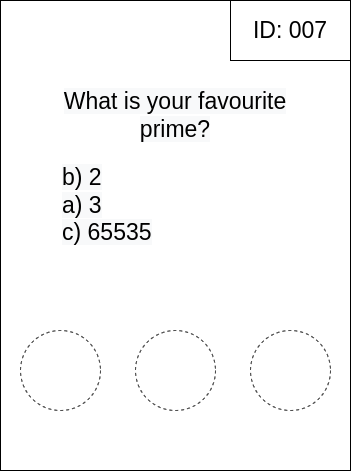
\includegraphics[width=0.3\textwidth]{../resources/high_level_ballot_top.drawio.png}
		\caption{Top half of ballot}
	\end{figure}
\end{frame}

\begin{frame}{Ballot layout: Bottom page}
	\begin{itemize}
		\item Bottom page has answer symbols (here: letters)
		\item Order of these is randomised per ballot
		\item Symbols can be seen through cutouts in top page
	\end{itemize}
	\begin{figure}
		\centering
		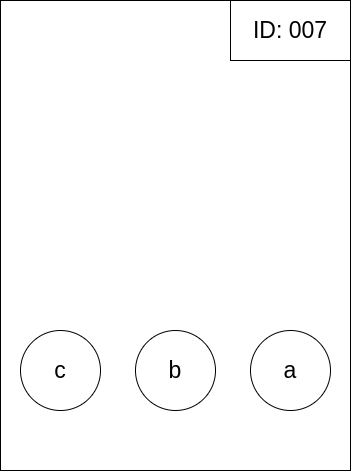
\includegraphics[width=0.3\textwidth]{../resources/high_level_ballot_bottom.drawio.png}
		\caption{Bottom half of ballot}
	\end{figure}
\end{frame}

\section{Voting process}

\begin{frame}{Voting process: Voting}
	\begin{itemize}
		\item Voter receives ballot, both pages stacked atop each other
		\item Voter marks their choice using a dauber (huge highlighter)
		\item This leaves stain on both top and bottom page
	\end{itemize}
	\begin{figure}
		\centering
		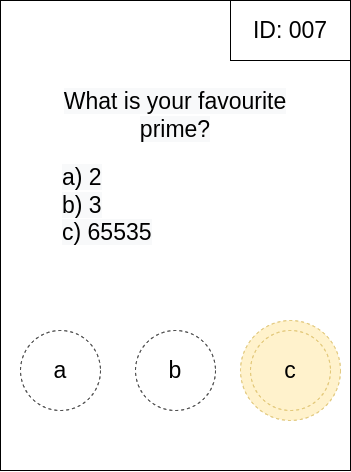
\includegraphics[width=0.3\textwidth]{../resources/high_level_ballot_voted.drawio.png}
		\caption{Ballot after voting}
	\end{figure}
\end{frame}

\begin{frame}{Voting process: Scanning}
	\begin{itemize}
		\item Voter destroys one half of the ballot
		\item Other half gets scanned, and kept by voter as receipt
		\item Unable to learn vote by looking at one half only
		\item But: What to do in tally phase? Someone must know the
			permutations of questions and answers.
	\end{itemize}
	\begin{figure}
		\centering
		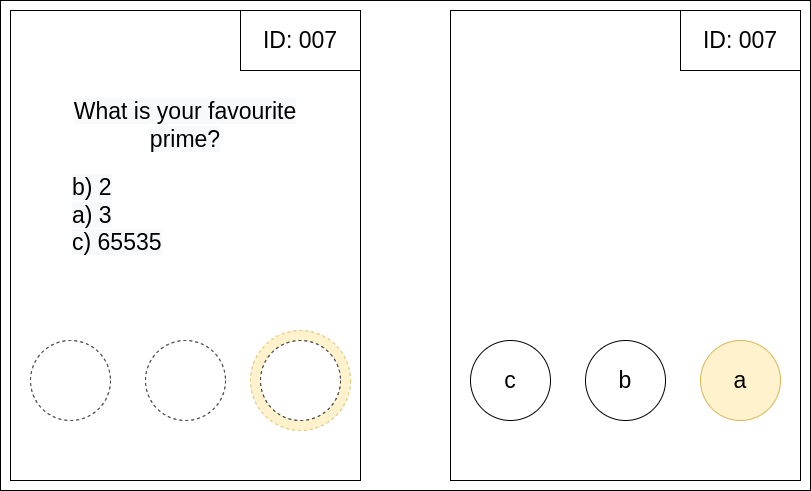
\includegraphics[width=0.65\textwidth]{../resources/high_level_ballot_voted_split.drawio.png}
		\caption{Top (left) and bottom (right) halves of ballot after voting}
	\end{figure}
\end{frame}

\section{Setup phase}

\begin{frame}{Election setup}
	Election authority defines three tables:
	\begin{itemize}
		\item \textbf{P}: Print. Data which ends up on ballot.
		\item \textbf{D}: Decrypt. Required to decrypt votes.
		\item \textbf{R}: Results.
		\item For following examples: Assume question with two choices:
			$(a, b)$.
	\end{itemize}
\end{frame}

\begin{frame}{Setup: Print table}
	\begin{center}
		\begin{tabular}{|c|c|c|c|c|c|}
			\hline
			$ID_P$ & $\pi_{top}$ & $\pi_{bottom}$ & $Choice$ & $Com_{\pi_{top}}$ & $Com_{\pi_{bottom}}$ \\
			\hline
			1 & ab & ab & & $C_{1, 1}$ & $C_{1, 2}$ \\
			2 & ab & ba & & $C_{2, 1}$ & $C_{2, 2}$ \\
			3 & ba & ab & & $C_{3, 1}$ & $C_{3, 2}$ \\
			4 & ba & ba & & $C_{4, 1}$ & $C_{4, 2}$ \\
			5 & ab & ba & & $C_{5, 1}$ & $C_{5, 2}$ \\
			6 & ba & ab & & $C_{6, 1}$ & $C_{6, 2}$ \\
			\hline
		\end{tabular}
	\end{center}

	\begin{itemize}
		\item $\pi_{top}, \pi_{bottom}$ are random permutations of top and bottom
			sheet, here shown explicitly.
		\item $Com_{\pi_{top}}, Com_{\pi_{bottom}}$ cryptographic commitments to
			$\pi_{top}$, $\pi_{bottom}$
		\item Consider ballot $1$ as canonical, i.e.
			$\pi_{top} = \pi_{bottom} = id$.
	\end{itemize}
\end{frame}

\begin{frame}{Setup: Decryption table}
	\begin{columns}
		\column{0.3\textwidth}
		\begin{center}
			\begin{tabular}{|c|c|c|}
				\hline
				$ID_P$ & $\pi_{top}$ & $\pi_{bottom}$ \\
				\hline
				1 & ab & ab \\
				2 & ab & ba \\
				3 & ba & ab \\
				4 & ba & ba \\
				5 & ab & ba \\
				6 & ba & ab \\
				\hline
			\end{tabular}
		\end{center}

		\column{0.7\textwidth}
		\begin{center}
			\begin{tabular}{|c|c|c|c|c|c|}
				\hline
				$ID_P$ & $\pi_1$ & $\hat{R}$ & $\pi_2$ & $ID_R$ & $Com_{i}$ \\
				\hline
				6 & $\rightarrow$       & & $\circlearrowright$ & 5 & $C_6$ \\
				5 & $\circlearrowright$ & & $\rightarrow$       & 4 & $C_5$ \\
				2 & $\circlearrowright$ & & $\rightarrow$       & 1 & $C_2$ \\
				1 & $\circlearrowright$ & & $\circlearrowright$ & 3 & $C_1$ \\
				4 & $\rightarrow$       & & $\rightarrow$       & 2 & $C_4$ \\
				3 & $\rightarrow$       & & $\circlearrowright$ & 6 & $C_3$ \\
				\hline
				\multicolumn{2}{|c|}{$Com_{ID_P, \pi_1}$} &   & \multicolumn{2}{c|}{$Com_{\pi_2, ID_R}$} & \\
				\hline
			\end{tabular}
		\end{center}
	\end{columns}

	\begin{itemize}
		\item $\pi_1, \pi_2$ are permutations, but \textbf{not}
			equal to permutations of top / bottom sheet. Rather
			$\pi_{top} \circ \pi_{bottom} \circ \pi_1 \circ \pi_2 = id$.
		\item $\rightarrow$ is identity permutation,
			$\circlearrowright$ non-identity permutation on two
			elements.
		\item $Com_{i}$ is commitment to row, $Com_{ID_P, \pi_1},
			Com_{\pi_2, ID_R}$ to two columns respectively.
	\end{itemize}
\end{frame}

\begin{frame}{Setup: Results table}
	\begin{center}
		\begin{tabular}{|c|c|}
			\hline
			$ID_R$ & $R$ \\
			\hline
			1 & \\
			2 & \\
			3 & \\
			4 & \\
			5 & \\
			6 & \\
			\hline
		\end{tabular}
	\end{center}

	\begin{itemize}
		\item Results table is empty, as outcome is not known ahead of
			the election.\footnote{Does not apply to certain
			countries}
	\end{itemize}
\end{frame}

\begin{frame}{Setup: Audit}
	\begingroup
	\fontsize{8pt}{10pt}\selectfont
	\begin{columns}
		\column{0.5\textwidth}
		\begin{center}
			\begin{tabular}{|c|c|c|c|c|c|}
				\hline
				$ID_P$ & $\pi_{t}$ & $\pi_{b}$ & $c$ & $Com_{\pi_{t}}$ & $Com_{\pi_{b}}$ \\
				\hline
				1 & & & & $C_{1, 1}$ & $C_{1, 2}$ \\
				2 & & & & $C_{2, 1}$ & $C_{2, 2}$ \\
				3 & & & & $C_{3, 1}$ & $C_{3, 2}$ \\
				4 & & & & $C_{4, 1}$ & $C_{4, 2}$ \\
				5 & & & & $C_{5, 1}$ & $C_{5, 2}$ \\
				6 & & & & $C_{6, 1}$ & $C_{6, 2}$ \\
				\hline
			\end{tabular}
		\end{center}

		\column{0.5\textwidth}
		\begin{center}
			\begin{tabular}{|c|c|c|c|c|c|}
				\hline
				$ID_P$ & $\pi_1$ & $\hat{R}$ & $\pi_2$ & $ID_R$ & $Com_{i}$ \\
				\hline
				& & & & & $C_6$ \\
				& & & & & $C_5$ \\
				& & & & & $C_2$ \\
				& & & & & $C_1$ \\
				& & & & & $C_4$ \\
				& & & & & $C_3$ \\
				\hline
				\multicolumn{2}{|c|}{$Com_{ID_P, \pi_1}$} &   & \multicolumn{2}{c|}{$Com_{\pi_2, ID_R}$} & \\
				\hline
			\end{tabular}
		\end{center}
	\end{columns}
	\endgroup

	\begin{itemize}
		\item Commitments of P and D tables released to the public.
	\end{itemize}
\end{frame}

\begin{frame}{Setup: Audit (cont)}
	\begingroup
	\fontsize{8pt}{10pt}\selectfont
	\begin{columns}
		\column{0.5\textwidth}
		\begin{center}
			\begin{tabular}{|c|c|c|c|c|c|}
				\hline
				$ID_P$ & $\pi_{t}$ & $\pi_{b}$ & $c$ & $Com_{\pi_{t}}$ & $Com_{\pi_{b}}$ \\
				\hline
				1 & & & & $C_{1, 1}$ & $C_{1, 2}$ \\
				2 & ab & ba & & $C_{2, 1}$ & $C_{2, 2}$ \\
				3 & & & & $C_{3, 1}$ & $C_{3, 2}$ \\
				4 & ba & ba & & $C_{4, 1}$ & $C_{4, 2}$ \\
				5 & ab & ba & & $C_{5, 1}$ & $C_{5, 2}$ \\
				6 & & & & $C_{6, 1}$ & $C_{6, 2}$ \\
				\hline
			\end{tabular}
		\end{center}

		\column{0.5\textwidth}
		\begin{center}
			\begin{tabular}{|c|c|c|c|c|c|}
				\hline
				$ID_P$ & $\pi_1$ & $\hat{R}$ & $\pi_2$ & $ID_R$ & $Com_{i}$ \\
				\hline
				  &                     & &                     &   & $C_6$ \\
				5 & $\circlearrowright$ & & $\rightarrow$       & 4 & $C_5$ \\
				2 & $\circlearrowright$ & & $\rightarrow$       & 1 & $C_2$ \\
				  &                     & &                     &   & $C_1$ \\
				4 & $\rightarrow$       & & $\rightarrow$       & 2 & $C_4$ \\
				  &                     & &                     &   & $C_3$ \\
				\hline
				\multicolumn{2}{|c|}{$Com_{ID_P, \pi_1}$} &   & \multicolumn{2}{c|}{$Com_{\pi_2, ID_R}$} & \\
				\hline
			\end{tabular}
		\end{center}
	\end{columns}
	\endgroup

	\begin{itemize}
		\item Auditors pick half the rows to reveal
		\item Can then verify row commitments, and $\pi_t \circ \pi_b
			\circ \pi_1 \circ \pi_2 = id$
		\item Remaining ballots are then printed
	\end{itemize}
\end{frame}

\section{Voting phase}

\begin{frame}{Voting: Filling out ballots}
	To recap:
	\begin{itemize}
		\item Voter gets ballot, marks their choice
		\item Voter destroys one of the two pages
		\item Other page is scanned and given to voter as receipt
		\item Voter's permuted choice stored in $Choice$ column of P table.
		\item \emph{Caveat}: Voters are supposed to verify that printed
			ballot matches one of the unspoiled commitments from P
			table. Paper does not describe how that is intended to
			be done.
	\end{itemize}
\end{frame}

\begin{frame}{Voting: Decrypting votes}
	\begin{columns}
		\column{0.5\textwidth}
		\begin{center}
			\begin{tabular}{|c|c|c|c|}
				\hline
				$ID_P$ & $\pi_{top}$ & $\pi_{bottom}$ & $Choice$ \\
				\hline
				1 & ab &    & a (= a) \\
				3 &    & ab & b (= a) \\
				6 & ba &    & a (= b) \\
				\hline
			\end{tabular}
		\end{center}
		\column{0.5\textwidth}
		\begin{center}
			\begin{tabular}{|c|c|c|c|c|}
				\hline
				$ID_P$ & $\pi_1$ & $\hat{R}$ & $\pi_2$ & $ID_R$ \\
				\hline
				6 & $\rightarrow$       & a & $\circlearrowright$ & 5 \\
				1 & $\circlearrowright$ & b & $\circlearrowright$ & 3 \\
				3 & $\rightarrow$       & b & $\circlearrowright$ & 6 \\
				\hline
			\end{tabular}
		\end{center}
	\end{columns}

	\begin{itemize}
		\item P table now only has information of scanned ballots
		\item $Choice$ is encrypted vote. In brackets (unknown to election
			authority!) is plaintext vote
		\item Election authority calculates $\hat{R} = \pi_1(Choice)$
	\end{itemize}
\end{frame}

\begin{frame}{Voting: Decrypting votes (cont)}
	\begin{columns}
		\column{0.5\textwidth}
		\begin{center}
			\begin{tabular}{|c|c|c|c|c|}
				\hline
				$ID_P$ & $\pi_1$ & $\hat{R}$ & $\pi_2$ & $ID_R$ \\
				\hline
				6 & $\rightarrow$       & a & $\circlearrowright$ & 5 \\
				1 & $\circlearrowright$ & b & $\circlearrowright$ & 3 \\
				3 & $\rightarrow$       & b & $\circlearrowright$ & 6 \\
				\hline
			\end{tabular}
		\end{center}
		\column{0.5\textwidth}
		\begin{center}
			\begin{tabular}{|c|c|}
				\hline
				$ID_R$ & $R$ \\
				\hline
				3 & a \\
				5 & b \\
				6 & a \\
				\hline
			\end{tabular}
		\end{center}
	\end{columns}

	\begin{itemize}
		\item Election authority calculates $R = \pi_2(\hat{R}) =
			(\pi_2 \circ \pi_1)(choice)$
		\item If voter chose $m$, then $Choice = (\pi_{top} \circ
			\pi_{bottom})(m)$, and as $\pi_{2} \circ \pi_{1}
			\circ \pi_{top} \circ \pi_{bottom} = id$, $R = m$.
		\item Election authority can now publish the results of the election
	\end{itemize}
\end{frame}

\begin{frame}{Voting: Decryption audit}
	\begin{columns}
		\column{0.25\textwidth}
		\begin{center}
			\begin{tabular}{|c|c|}
				\hline
				$ID_P$ & $C$ \\
				\hline
				1 & a \\
				3 & b \\
				6 & a \\
				\hline
			\end{tabular}
		\end{center}
		\column{0.5\textwidth}
		\begin{center}
			\begin{tabular}{|c|c|c|c|c|}
				\hline
				$ID_P$ & $\pi_1$ & $\hat{R}$ & $\pi_2$ & $ID_R$ \\
				\hline
				  &                     & a &                     &   \\
				  &                     & b &                     &   \\
				  &                     & b &                     &   \\
				\hline
				\multicolumn{2}{|c|}{$Com_{ID_P, \pi_1}$} &   & \multicolumn{2}{c|}{$Com_{\pi_2, ID_R}$} \\
				\hline
			\end{tabular}
		\end{center}
		\column{0.25\textwidth}
		\begin{center}
			\begin{tabular}{|c|c|}
				\hline
				$ID_R$ & $R$ \\
				\hline
				3 & a \\
				5 & b \\
				6 & a \\
				\hline
			\end{tabular}
		\end{center}
	\end{columns}

	\begin{itemize}
		\item Auditor gets to choose whether to reveal left or right half of decryption table
	\end{itemize}
\end{frame}

\begin{frame}{Voting: Decryption audit (cont)}
	\begin{columns}
		\column{0.25\textwidth}
		\begin{center}
			\begin{tabular}{|c|c|}
				\hline
				$ID_P$ & $C$ \\
				\hline
				1 & a \\
				3 & b \\
				6 & a \\
				\hline
			\end{tabular}
		\end{center}
		\column{0.5\textwidth}
		\begin{center}
			\begin{tabular}{|c|c|c|c|c|}
				\hline
				$ID_P$ & $\pi_1$ & $\hat{R}$ & $\pi_2$ & $ID_R$ \\
				\hline
				6 & $\rightarrow$       & a &                     &   \\
				1 & $\circlearrowright$ & b &                     &   \\
				3 & $\rightarrow$       & b &                     &   \\
				\hline
				\multicolumn{2}{|c|}{$Com_{ID_P, \pi_1}$} &   & \multicolumn{2}{c|}{$Com_{\pi_2, ID_R}$} \\
				\hline
			\end{tabular}
		\end{center}
		\column{0.25\textwidth}
		\begin{center}
			\begin{tabular}{|c|c|}
				\hline
				$ID_R$ & $R$ \\
				\hline
				3 & a \\
				5 & b \\
				6 & a \\
				\hline
			\end{tabular}
		\end{center}
	\end{columns}

	\begin{itemize}
		\item Assume left half revealed
		\item Auditor verifies that $\pi_1(C) = \hat{R}$
		\item And that column commitment $Com_{ID_P, \pi_1}$ holds
		\item Probability $1/2$ of catching cheating election authority
			\begin{itemize}
				\item Decryption table $D$ can be split into
					$n$ shards $D_1, \ldots, D_n$, for each
					of which auditor can choose the half to
					reveal.
			\end{itemize}
	\end{itemize}
\end{frame}

\begin{frame}{Voting: Cast-as-intended audit}
	\begin{itemize}
		\item Election authority also publishes the scans of the ballots online
		\item Voter can look it up using their ballot's serial number, and compare to their receipt
	\end{itemize}
\end{frame}

\begin{frame}{Voting: Voter privacy?}
	\begin{itemize}
		\item Only half the ballot public, thus unable to determine vote from $\pi_{top}, \pi_{bottom}$
		\item Only half the D table public, thus unable to determine vote from $\pi_1, \pi_2$
		\item Does not hold against malicious election authority, of course
	\end{itemize}
\end{frame}

\section{Some (theoretical) attacks on privacy}

\begin{frame}{Attacking permutations}
	\begin{itemize}
		\item Row commitments contain information about ballot
			permutations, thus commitment scheme must be hiding.
			\begin{itemize}
				\item Paper: Custom, complicated commitment
					scheme atop of AES and SHA-256. No
					proofs.
			\end{itemize}
		\item Row permutations of D and R tables must be irreversible
			\begin{itemize}
				\item Paper: Row permutations using AES with key known to election authority.
			\end{itemize}
	\end{itemize}
\end{frame}

\section{A gaping hole in ballot integrity}

\begin{frame}{Print table vs printed ballots}
	\begin{itemize}
		\item Audits in various phases of election have chance of
			catching cheating election authority
		\item Except: Verifying that P table equal to what is printed
			requires voters to verify commitments
		\item Cheating election authority has many other
			options\autocite{lundinTearDestroyChain2012}
	\end{itemize}
\end{frame}

\section{Vote-buying attack on older version of Punchscan \autocite{moranSplitballotVotingEverlasting2010}}

\begin{frame}{Vote-buying attack on older version of Punchscan}
	\begin{itemize}
		\item In first version, voter did not have to commit to which
			page to keep until after having voted.
		\item Consider an election between Alice and Bob
		\item We want to vote for Bob
		\item There is a coercing party wanting to help Alice
	\end{itemize}
\end{frame}

\begin{frame}{Vote-buying attack on older version of Punchscan (cont)}
	\begin{figure}
		\centering
		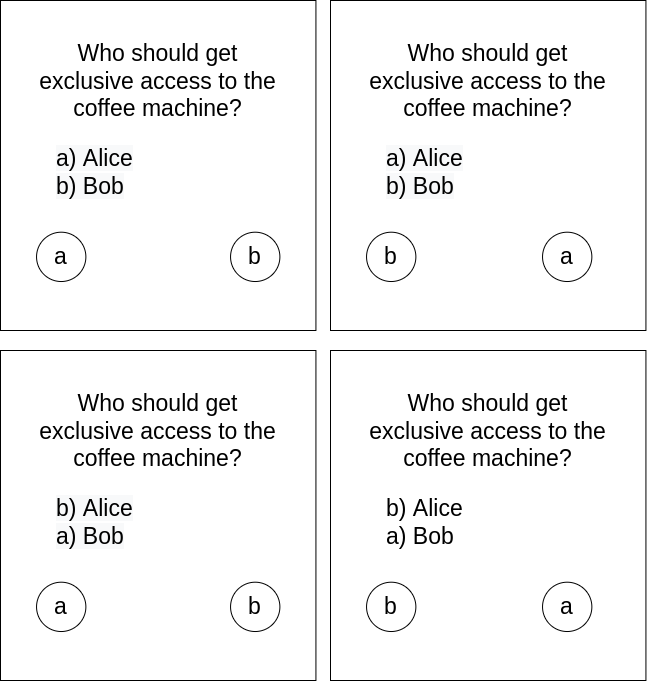
\includegraphics[width=0.55\textwidth]{../resources/vote_buying.drawio.png}
		\caption{Possible ballots}
	\end{figure}
\end{frame}

\begin{frame}{Vote-buying attack on older version of Punchscan (cont)}
	\begin{figure}
		\centering
		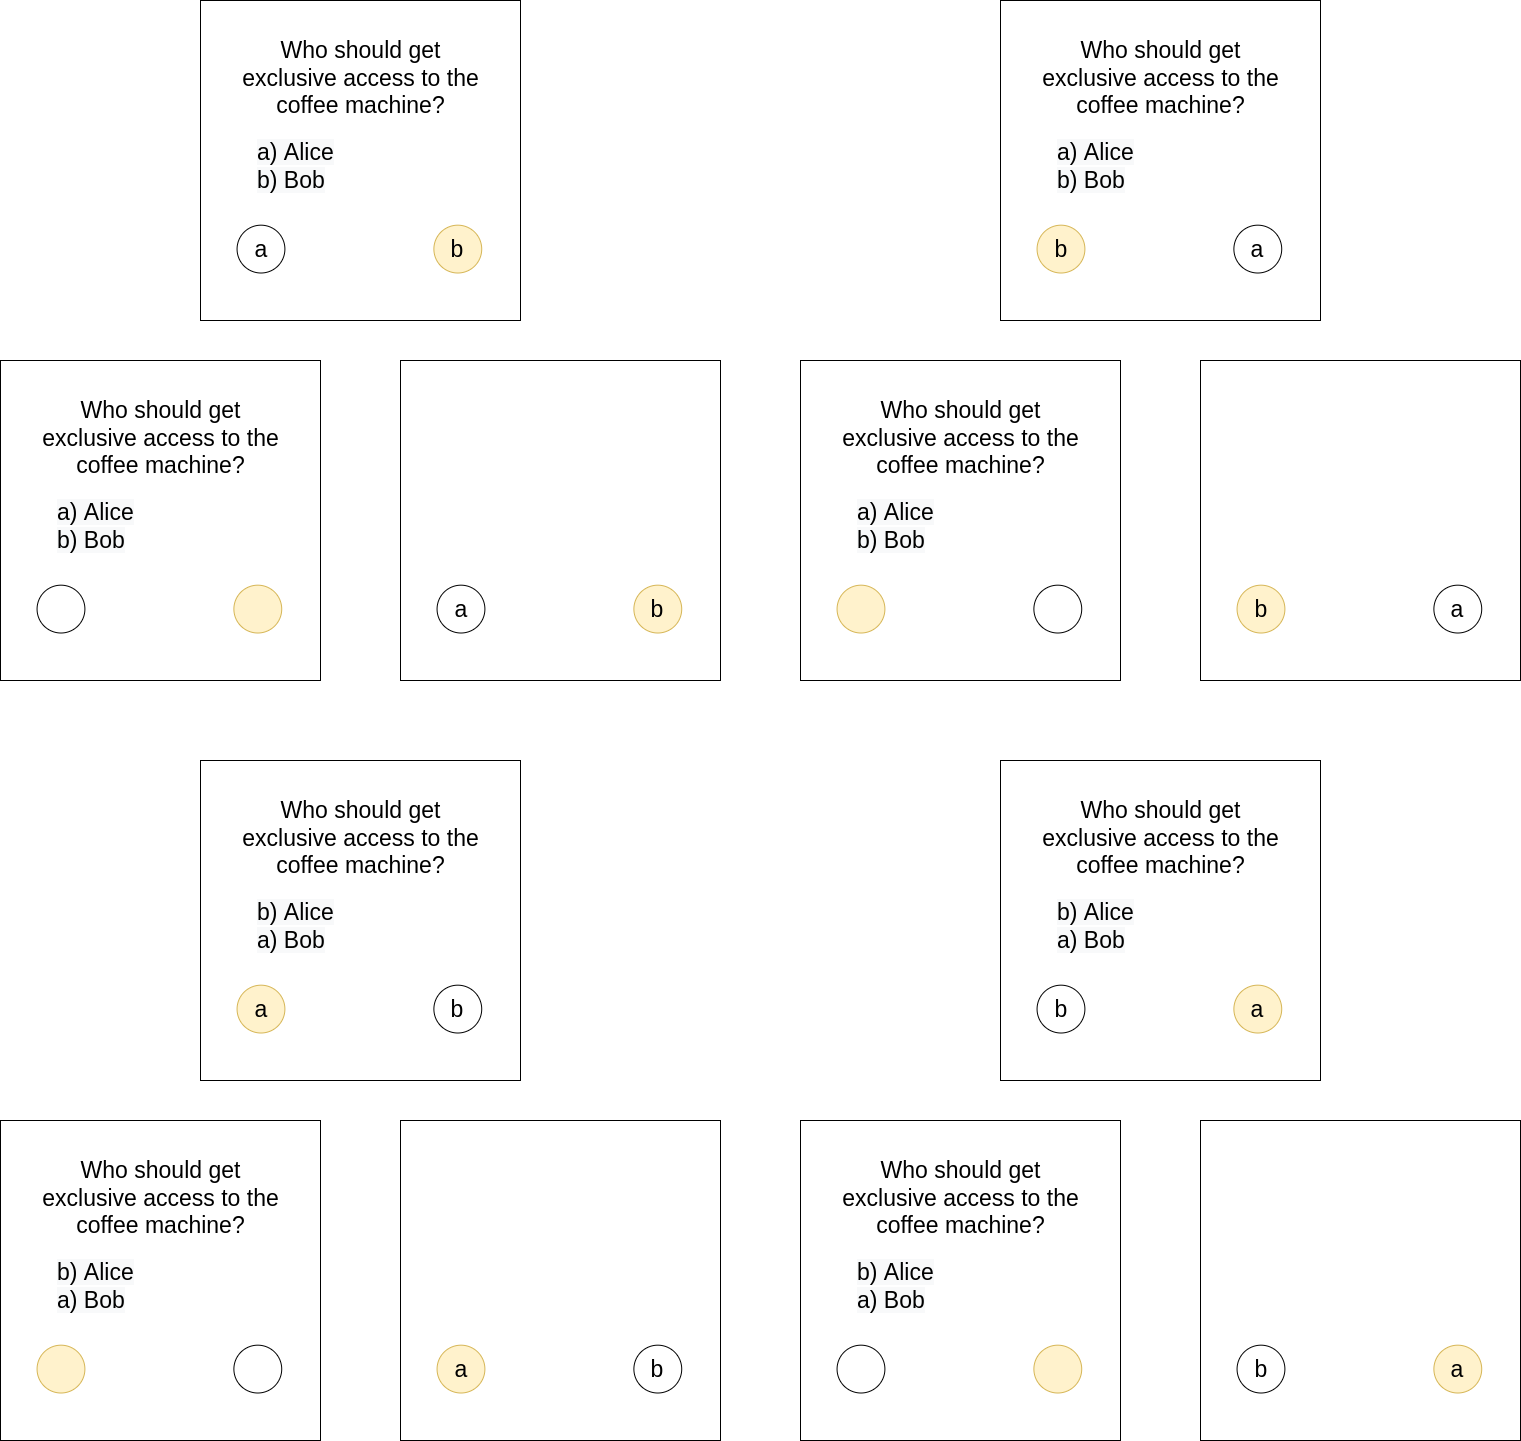
\includegraphics[width=0.65\textwidth]{../resources/vote_buying_split.drawio.png}
		\caption{Possible ballot layouts when voting for Bob}
	\end{figure}
\end{frame}

\begin{frame}{Vote-buying attack on older version of Punchscan (cont)}
	\textbf{As a coercing party, we now offer to pay for any ballot receipt, as long as:}
	\begin{itemize}
		\item It is not a ballot where the order is b -> a
		\item Where the voter selected the second option
	\end{itemize}
\end{frame}

\begin{frame}{Vote-buying attack on older version of Punchscan (cont)}
	\begin{figure}
		\centering
		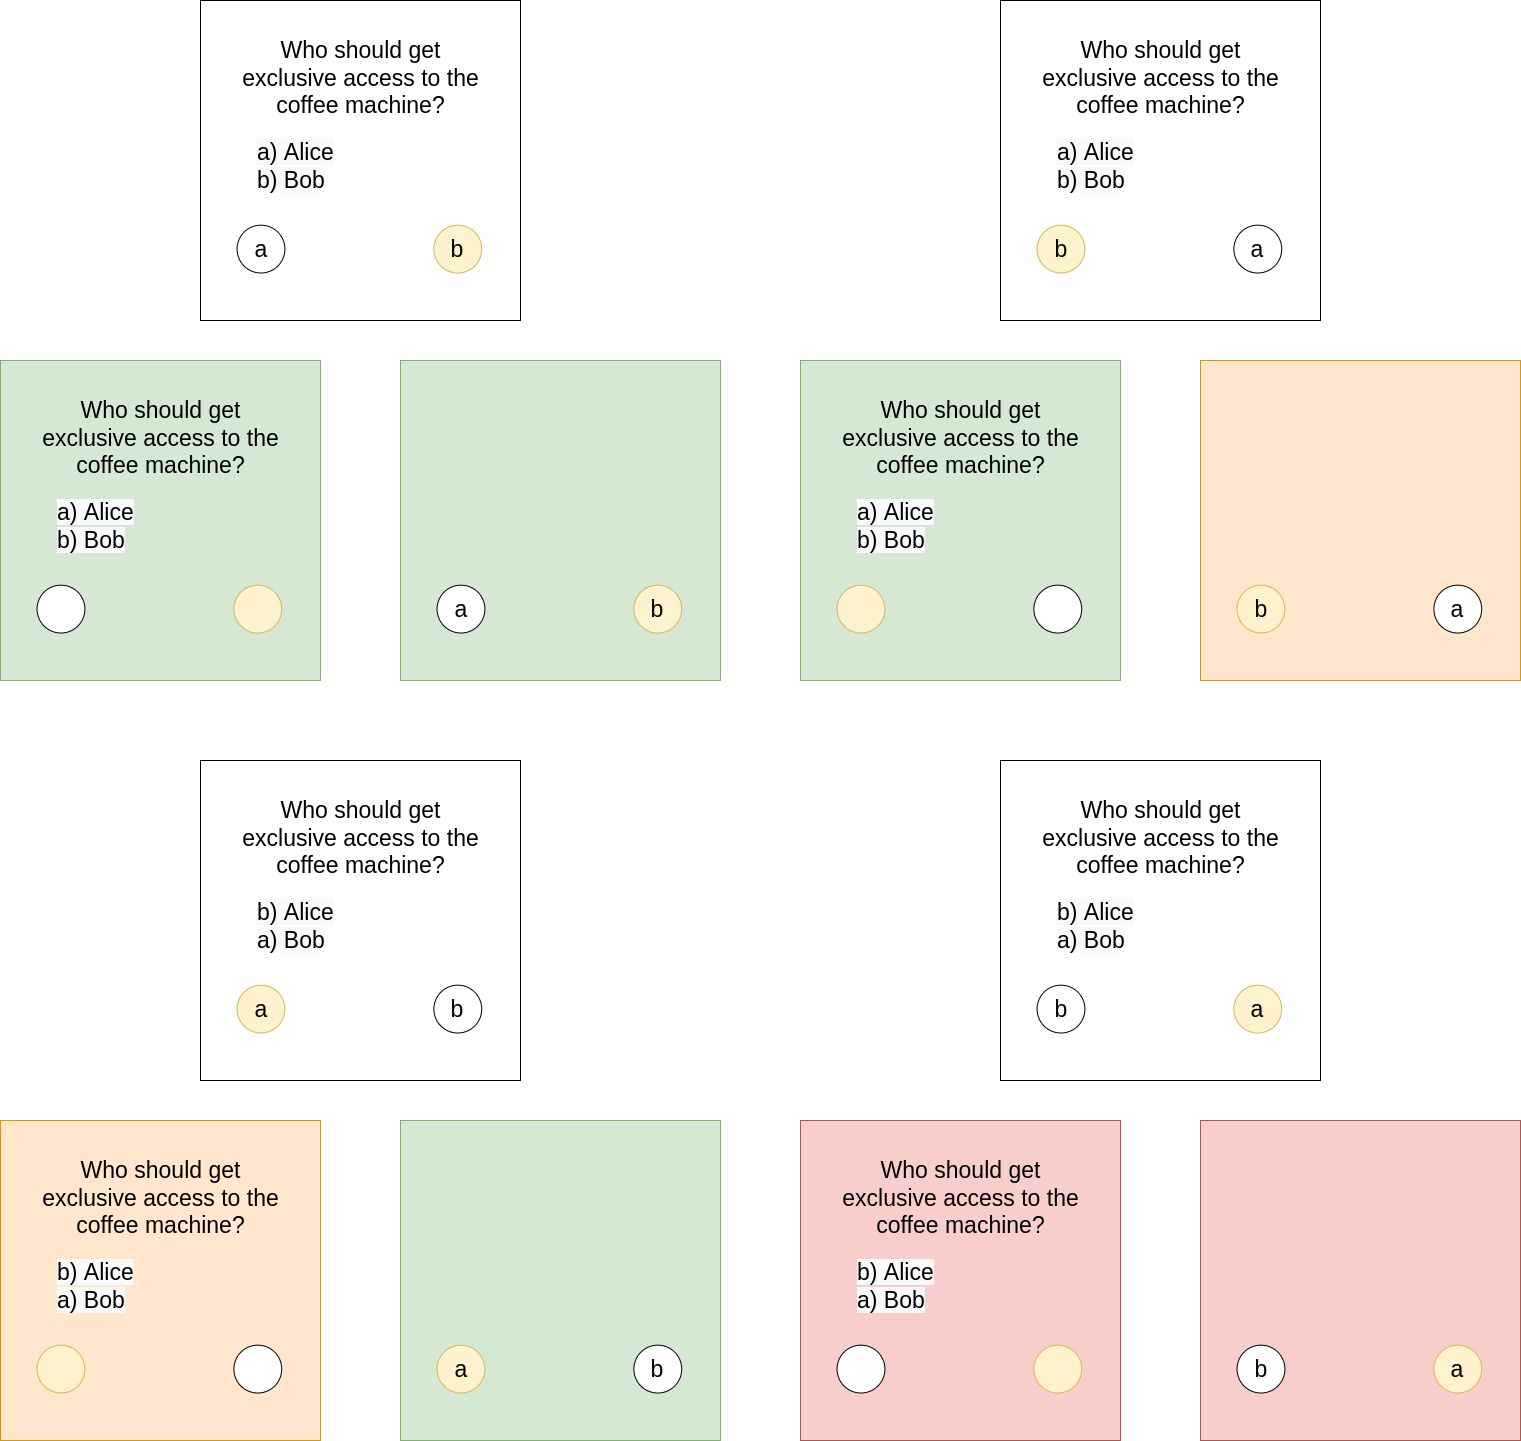
\includegraphics[width=0.65\textwidth]{../resources/vote_buying_split_highlighted.drawio.png}
		\caption{Possible ballot layouts when voting for Bob, accepted by coercer}
	\end{figure}
\end{frame}

\begin{frame}{Vote-buying attack on older version of Punchscan (cont)}
	\begin{figure}
		\centering
		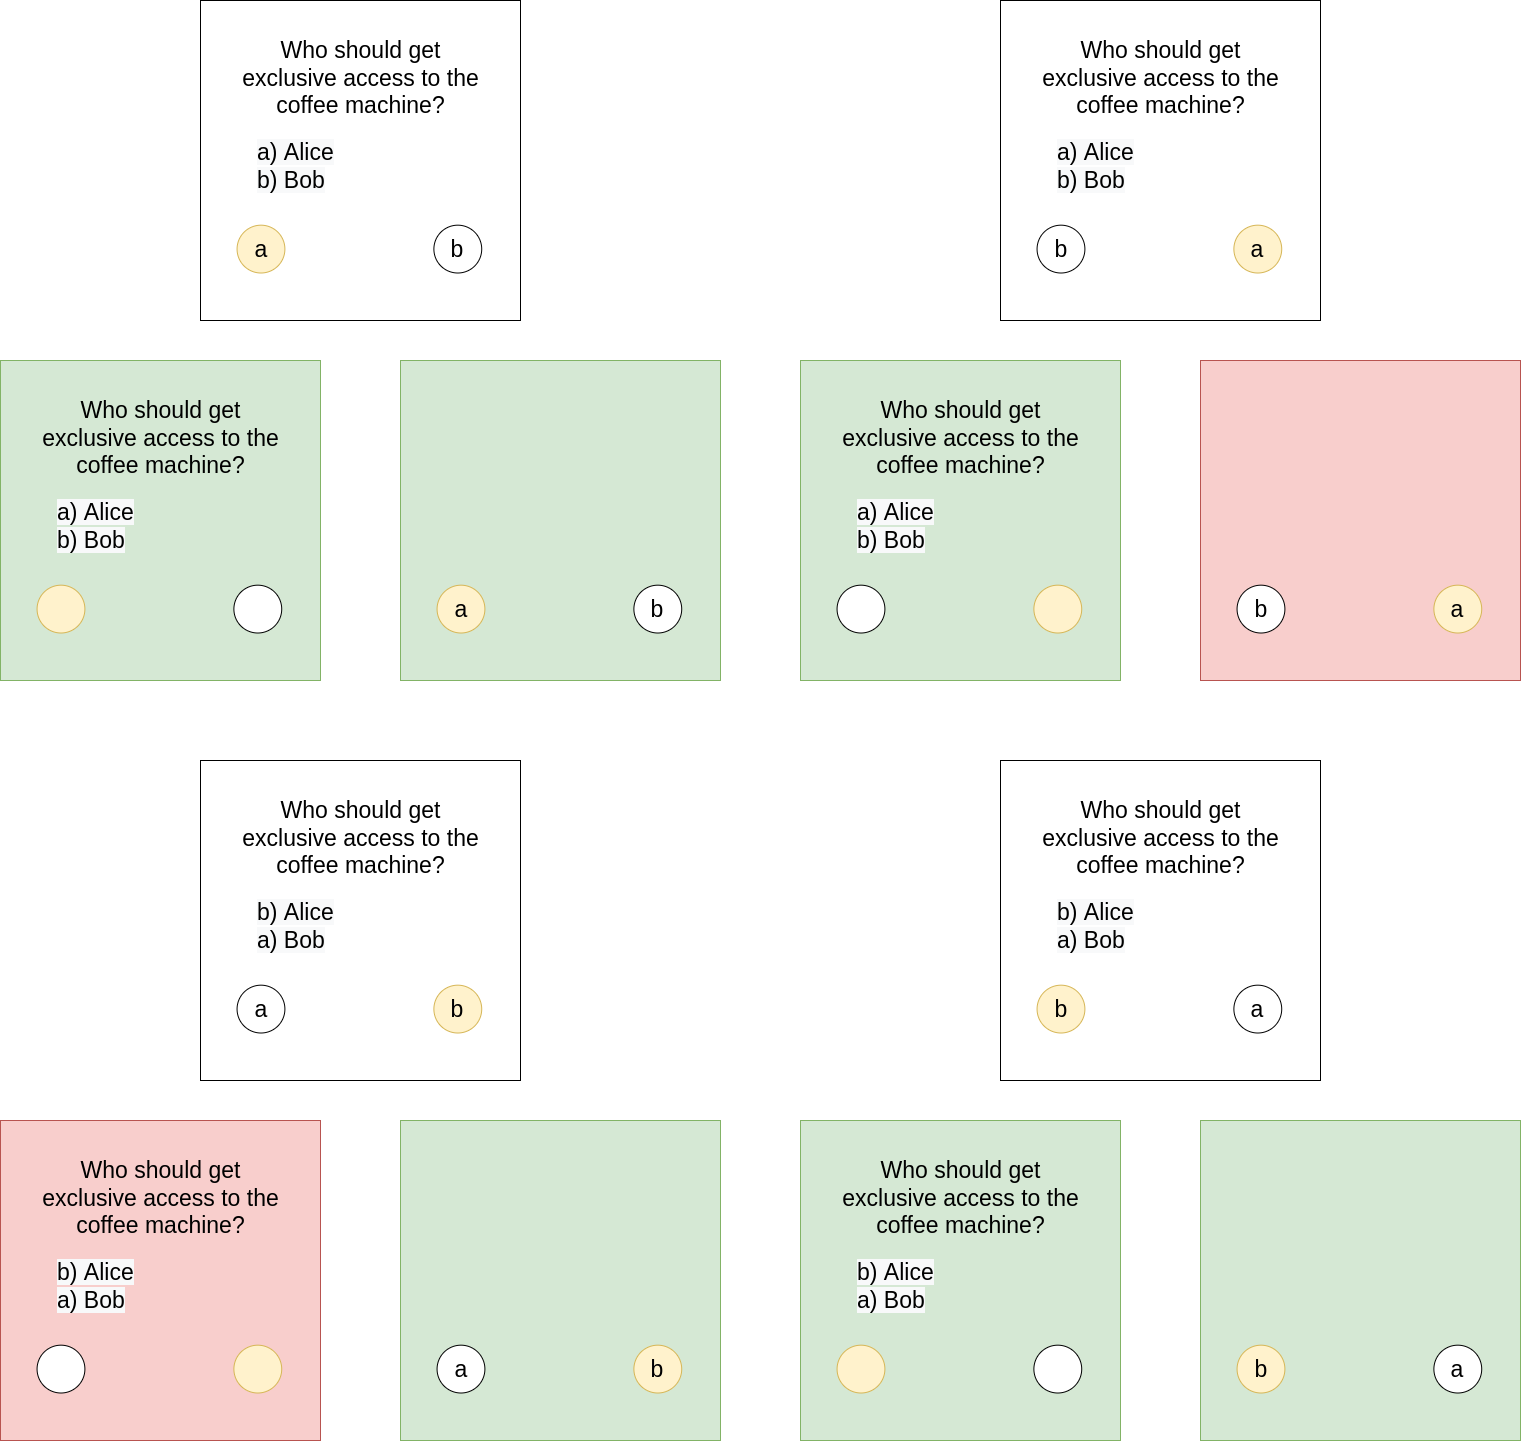
\includegraphics[width=0.65\textwidth]{../resources/vote_buying_split_highlighted_alice.drawio.png}
		\caption{Possible ballot layouts when voting for Alice, accepted by coercer}
	\end{figure}
\end{frame}

\begin{frame}{Vote-buying attack on older version of Punchscan (cont)}
	\begin{itemize}
		\item Fix in Punchscan: Voter must commit to which half to keep before seeing their ballot.
		\item Now, for every two Bob-voters we pay to vote for Alice...
		\item We also pay two Alice-voters to vote for Bob.
		\item Attack also extended to multi-candidate votes\autocite{kelseyAttackingPaperBasedE2E2010}
		\item This shows the importance of formal proofs, of which Punchscan has none.
	\end{itemize}
\end{frame}

\section{Summary}

\begin{frame}{Summary}
	\begin{itemize}
		\item Punchscan: Voter-verifiable election system with paper-based receipt
		\item No possibility for vote-buying --- except when it does
		\item Secure against a malicious election authority --- except when it is not
		\item Good example of difficulty in designing usable and
			secure system
	\end{itemize}
\end{frame}

\section{References}

\begin{frame}[allowframebreaks]
	\frametitle{References}
	\printbibliography
\end{frame}


\end{document}
